%% Creator: Inkscape 0.91, www.inkscape.org
%% PDF/EPS/PS + LaTeX output extension by Johan Engelen, 2010
%% Accompanies image file 'Histogram.pdf' (pdf, eps, ps)
%%
%% To include the image in your LaTeX document, write
%%   \input{<filename>.pdf_tex}
%%  instead of
%%   \includegraphics{<filename>.pdf}
%% To scale the image, write
%%   \def\svgwidth{<desired width>}
%%   \input{<filename>.pdf_tex}
%%  instead of
%%   \includegraphics[width=<desired width>]{<filename>.pdf}
%%
%% Images with a different path to the parent latex file can
%% be accessed with the `import' package (which may need to be
%% installed) using
%%   \usepackage{import}
%% in the preamble, and then including the image with
%%   \import{<path to file>}{<filename>.pdf_tex}
%% Alternatively, one can specify
%%   \graphicspath{{<path to file>/}}
%%
%% For more information, please see info/svg-inkscape on CTAN:
%%   http://tug.ctan.org/tex-archive/info/svg-inkscape
%%
\begingroup%
  \makeatletter%
  \providecommand\color[2][]{%
    \errmessage{(Inkscape) Color is used for the text in Inkscape, but the package 'color.sty' is not loaded}%
    \renewcommand\color[2][]{}%
  }%
  \providecommand\transparent[1]{%
    \errmessage{(Inkscape) Transparency is used (non-zero) for the text in Inkscape, but the package 'transparent.sty' is not loaded}%
    \renewcommand\transparent[1]{}%
  }%
  \providecommand\rotatebox[2]{#2}%
  \ifx\svgwidth\undefined%
    \setlength{\unitlength}{337.32282383bp}%
    \ifx\svgscale\undefined%
      \relax%
    \else%
      \setlength{\unitlength}{\unitlength * \real{\svgscale}}%
    \fi%
  \else%
    \setlength{\unitlength}{\svgwidth}%
  \fi%
  \global\let\svgwidth\undefined%
  \global\let\svgscale\undefined%
  \makeatother%
  \begin{picture}(1,0.28459414)%
    \put(0.18760426,0.27510725){\color[rgb]{0,0,0}\makebox(0,0)[b]{\smash{\textbf A)}}}%
    \put(0.78050908,0.27510725){\color[rgb]{0,0,0}\makebox(0,0)[b]{\smash{\textbf B)}}}%
    \put(0.34175925,0.00017967){\color[rgb]{0,0,0}\makebox(0,0)[b]{\smash{\footnotesize 255}}}%
    \put(0.37733348,0.02845956){\color[rgb]{0,0,0}\makebox(0,0)[lb]{\smash{\footnotesize $I$}}}%
    \put(0.02159119,0.25613433){\color[rgb]{0,0,0}\makebox(0,0)[rb]{\smash{\footnotesize $p$}}}%
    \put(0.03557423,0.00000017){\color[rgb]{0,0,0}\makebox(0,0)[rb]{\smash{}}}%
    \put(0.03346664,0.00017967){\color[rgb]{0,0,0}\makebox(0,0)[b]{\smash{\footnotesize 0}}}%
    \put(0.37733348,0.24546206){\color[rgb]{0,0,0}\makebox(0,0)[lb]{\smash{\footnotesize slab\'{y} kontrast}}}%
    \put(0.36760036,0.20633055){\color[rgb]{0,0,0}\makebox(0,0)[rb]{\smash{}}}%
    \put(0.37733348,0.22174562){\color[rgb]{0,0,0}\makebox(0,0)[lb]{\smash{\footnotesize n\'{i}zk\'{y} jas}}}%
    \put(0.37733348,0.19802947){\color[rgb]{0,0,0}\makebox(0,0)[lb]{\smash{\footnotesize vysok\'{y} jas}}}%
    \put(0.61449587,0.25613433){\color[rgb]{0,0,0}\makebox(0,0)[rb]{\smash{\footnotesize $p_{cum}$}}}%
    \put(0.93466392,0.00017967){\color[rgb]{0,0,0}\makebox(0,0)[b]{\smash{\footnotesize 255}}}%
    \put(0.97023815,0.02845956){\color[rgb]{0,0,0}\makebox(0,0)[lb]{\smash{\footnotesize $I$}}}%
    \put(0.62637131,0.00017967){\color[rgb]{0,0,0}\makebox(0,0)[b]{\smash{\footnotesize 0}}}%
    \put(0.60263779,0.20870203){\color[rgb]{0,0,0}\makebox(0,0)[rb]{\smash{\footnotesize $S_x \times S_y$}}}%
    \put(0,0){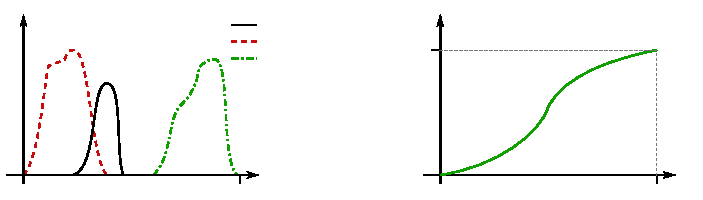
\includegraphics[width=\unitlength,page=1]{Histogram.pdf}}%
  \end{picture}%
\endgroup%
